%#MAKEINDEX makeindex interim01
\documentclass[10pt,a4j]{jarticle}

\input{include/macro.tex}
\input{include/preamble.tex}

\begin{document}
\begin{titlepage}

  \vspace*{25mm}

  \begin{center}
    {\huge 知能制御PBL\\}
    \vspace{5mm}
    {\Huge 第2回RCR中間報告\\}
    \vspace{20mm}
    {\Large 2017年5月31日}

    \vspace{25mm}

    {\LARGE 西田研究室\\}

    \vspace{10mm}

    {\Large
   13104042 烏谷崇大  \\
   14104043 桑野僚大  \\
   14104034 下松八重宏太\\
   14104090 中尾真人  \\
   14104111 本田空   \\
   14104131 山崎達也  \\
   16104313 山下翔   \\
}

  \end{center}

\end{titlepage}


\newpage
\section{目的}
学部3年までに学習した制御理論や電気回路,
情報工学の知識を使って, 競技場内を自律的に走行するロボットカーの製作を行う.
各研究室でチーム一丸となってプロジェクトを進行し,
共同で課題を達成することの難しさや楽しさを学び,
エンジニアとして仕事を進めるための素養を身に付ける.
情報工学の知識を使って, 競技場内を自律的に走行するロボットカーの製作を行う.
各研究室でチーム一丸となってプロジェクトを進行し,
共同で課題を達成することの難しさや楽しさを学び,


\section{Robot Car Race(RCR)2017競技ルール}
\subsection{ルール概要}
競技場には黄色のポールや,火災に見立てた複数の赤色のポールが設置されている.
ポールに接触せず,できるだけ速やかに火災を鎮火させる
消防ロボットカー(ロボカー)を作成する.

\subsection{競技場詳細}
競技場の全体図を図\ref{course}に示し,以下に詳細を説明する.
\begin{enumerate}
  \item 競技場は板張りの床であり,縦・横ともに $5400\unit{mm}$である.

  \item 競技場には黄色の固定ポールと赤色の火災ポールが設置されており,
        スタートからゴールまで,固定ポールには接触,
        火災ポールには衝突することなく通過しなければならない.

  \item 火災ポールは青色の鎮火ポールに赤色の幕を被せたものであり,
        上部におもりなどを落としたり,幕を剥がしたりすることで,
        鎮火ポールに変化させる(このポールの製作も行うこと).

  \item スタート後は右手に固定ポールを見ながら直進し,
        消火活動開始区間まで移動しなければならない.消火活動開始区間に
        進入後は,右折し,火災ポールを発見し次第,消火にあたる.

  \item すべての火災ポールを消火して,鎮火ポールに変化させたのち,
        ゴール地点で停止する.

  \item 火災ポールの配置は競技ごとに異なる.
        また,鎮火ポールが存在することもある.

  \item ポールは直径 $80\unit{mm}$・高さ $120\unit{mm}$の中空パイプであり,
        黄・赤・青の色が付けられている.
\end{enumerate}

\begin{figure}[t]
  \begin{center}
    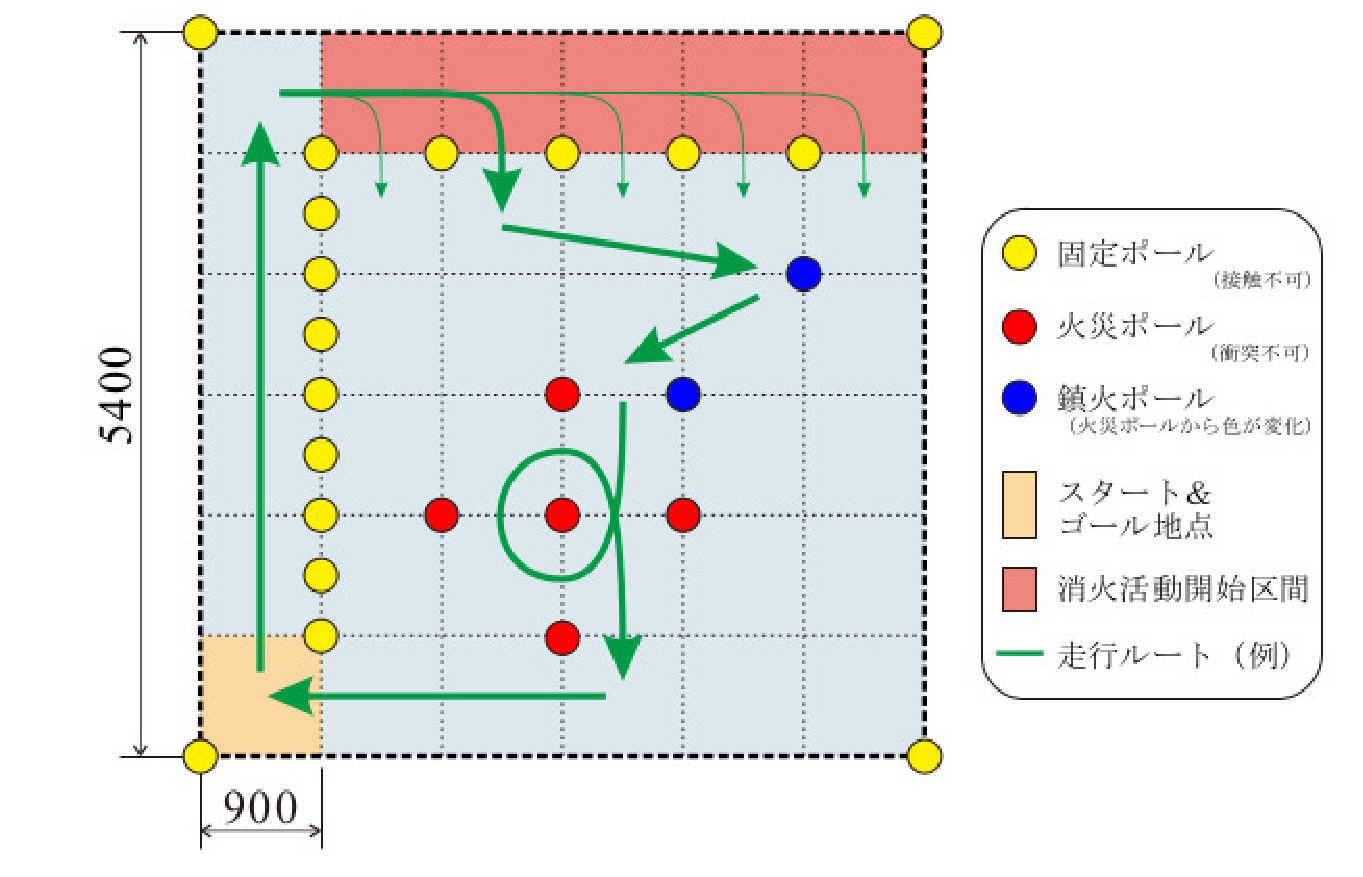
\includegraphics[width=1.0\hsize]{picture/course.eps}
    \caption{2017年度 RCR走行コース}
    \label{course}
  \end{center}
\end{figure}


\newpage
\section{ロボットカーの概要}
本年度のRCRでの我々の設計コンセプトは,
ロボットの安定した運用を可能にすることである,
そのために,ロボットカーには比較的構造が単純な独立二輪機構を採用する.
火災・鎮火ポールの判別は,ロボット前方に取り付けた単眼カメラの映像を
画像処理することで行う,また,PSD(Position Sensitive Detector)センサと
赤外線近接センサを用いてポールとロボットの距離を測定することで,
適切な軌道の走行とポールの消火を目指す.
製作にあたっては,研究室のメンバーをハードウェア,ソフトウェアの
担当に分けて進めることとする.


\section{消火について}
\subsection{消火ポール}
我々が用いる消火ポールは,以下のように製作する.\\
まず,塩化ビニル管に青い布を巻きつけて青いポールを作成する.
次に,青いポールの上から赤い布を覆うことで赤いポールとする.


\subsection{消火方法}
用いるポールの構造より,赤い布を青いポールから取り除くことで消火とする.
布を取り除く方法は,ロボットアームがポールの上から赤い布を
中に押し込んで,青いポールにするというものである.





\section{PSDセンサの同定実験}
\label{psdex}

前年度までに研究室で購入していた2種類のPSDセンサについて,
そのPSDセンサの精度を確かめるために同定実験を行った.

\subsection{センサの仕様}
前年度までに購入していた2種類のPSDセンサの仕様を以下に示す.
また,下記2つのセンサを便宜上,順に近距離センサ,遠距離センサと
呼ぶこととする.\\

 \begin{description}
  \item[【シャープ測距モジュール GP2Y0A21YK】] \mbox{} \\
	     測距範囲:$10〜80\unit{cm}$ \\
	     出力:アナログ電圧出力 \\
	     寸法:$29.5×13×13.5\unit{mm}$ \\
	     電源:$4.5〜5.5\unit{V}$
  \item[【シャープ測距モジュール GP2Y0A02YK】] \mbox{} \\
	     測距範囲:$20〜150\unit{cm}$ \\
	     出力:アナログ電圧出力 \\
	     寸法:$29.5×13×21.6\unit{mm}$ \\
	     電源:$4.5〜5.5\unit{V}$
 \end{description}


\subsection{実験装置}
PSDセンサの実験を行うため,図\ref{psded}のような実験装置を製作した.
PSDセンサは高さ$20\unit{mm}$の位置にセンサの発光部が左,
受光部が右になるように箱に水平に装着した.
PSDセンサを動作せるのにはArduino Unoを用い,
Arduino IDEのシリアルモニタを用いて出力電圧を測定した.
実験時のセンサとArduinoの配線を図\ref{psdwd}に,
Arduinoのプログラムを付録1に示す.
配線にはブレッドボードを用いた.また,ポールの代わりに,
ポールと同じ形状のスプレー缶を用いた.

\begin{figure}[t]
  \begin{center}
   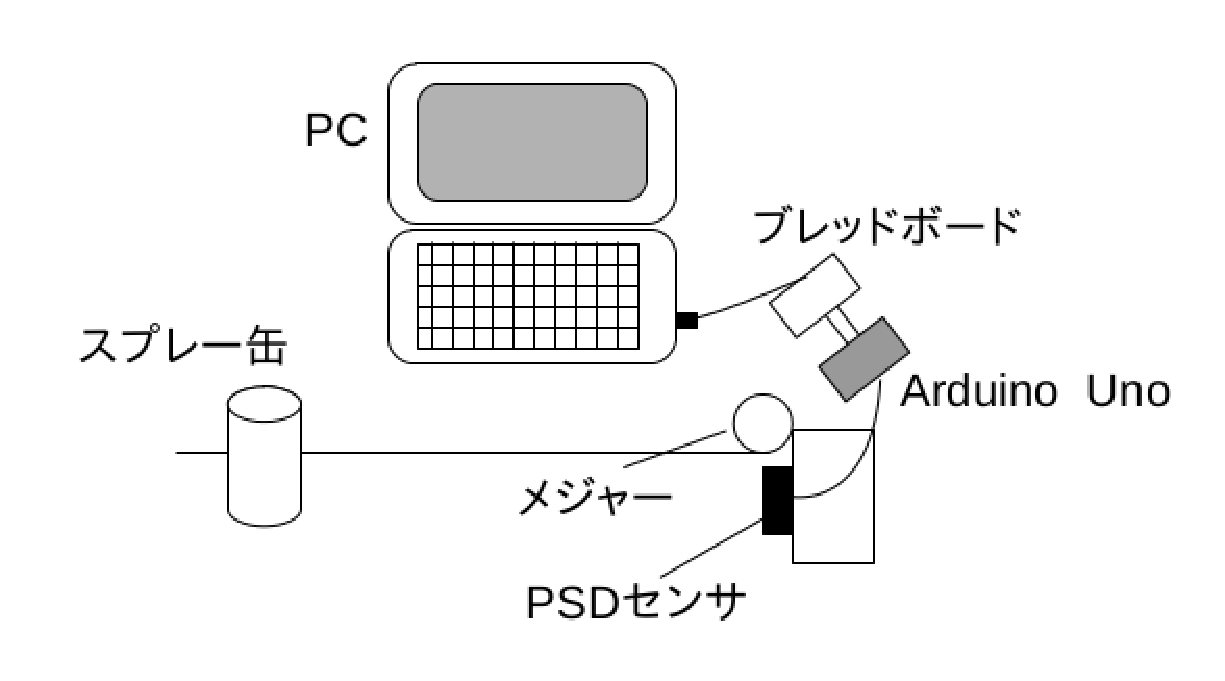
\includegraphics[scale = 0.8]{picture/psded.eps}
   \caption{PSD実験装置}
   \label{psded}
  \end{center}
\end{figure}

\begin{figure}
 \begin{center}   
  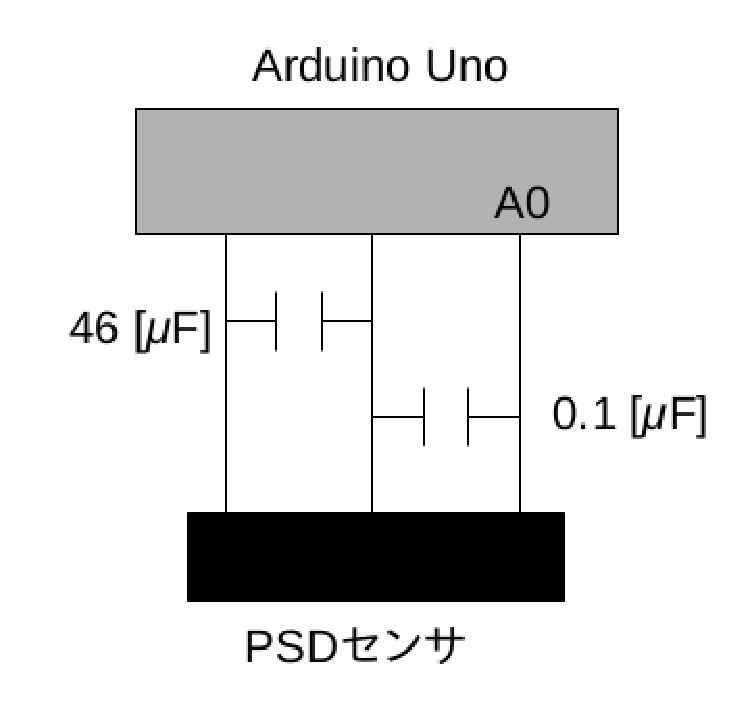
\includegraphics[scale = 0.8]{picture/psdwd.eps}
  \caption{PSDセンサの配線図}
  \label{psdwd}
 \end{center}
\end{figure}


\newpage
\subsection{実験方法}
PSDセンサの距離-出力電圧特性を測定するため以下の手順に従い実験を行った.
\begin{enumerate}
 \item PSDセンサの発光部・受光部の先端を距離$0\unit{cm}$とし,
       近距離センサは$5\unit{cm}$から$100\unit{cm}$まで,
       $5\unit{cm}$ずつスプレー缶を移動させ出力電圧を記録する.
       このとき,スプレー缶の中心はPSDセンサの中心の正面にくるように
       置き測定する.
 \item 先程と同様に,遠距離センサは$5\unit{cm}$から$170\unit{cm}$まで,
       $5\unit{cm}$ずつスプレー缶を移動させ出力電圧を記録する.
\end{enumerate} 

\subsection{実験結果}
縦軸を出力電圧,横軸をPSDセンサ-スプレー缶間の距離とし,
近距離センサの測定結果のグラフを図\ref{psdn}に,
遠距離センサの測定結果のグラフを図\ref{psdf}に示す.
図\ref{psdn}より,近距離センサは出力電圧が$40\unit{cm}$までは
滑らかに減少しており,$40\unit{cm}$からは大きな変化は見られない.
それに対して図\ref{psdf}より,遠距離センサは測距可能範囲内において
出力電圧が$80\unit{cm}$までは滑らかに減少しており,
$80\unit{cm}$からは変化に乏しいことがわかる.
よって,近距離センサでは$40\unit{cm}$以降,遠距離センサでは$80\unit{cm}$以降の距離を算出することが難しくなると考えられる.
ここで,今回のロボットは$40\unit{cm}$以降も距離を計測する必要がある.
従って適当なセンサは,遠距離センサであると考えられる.


\newpage
\begin{figure}[htb]
  \begin{center}
    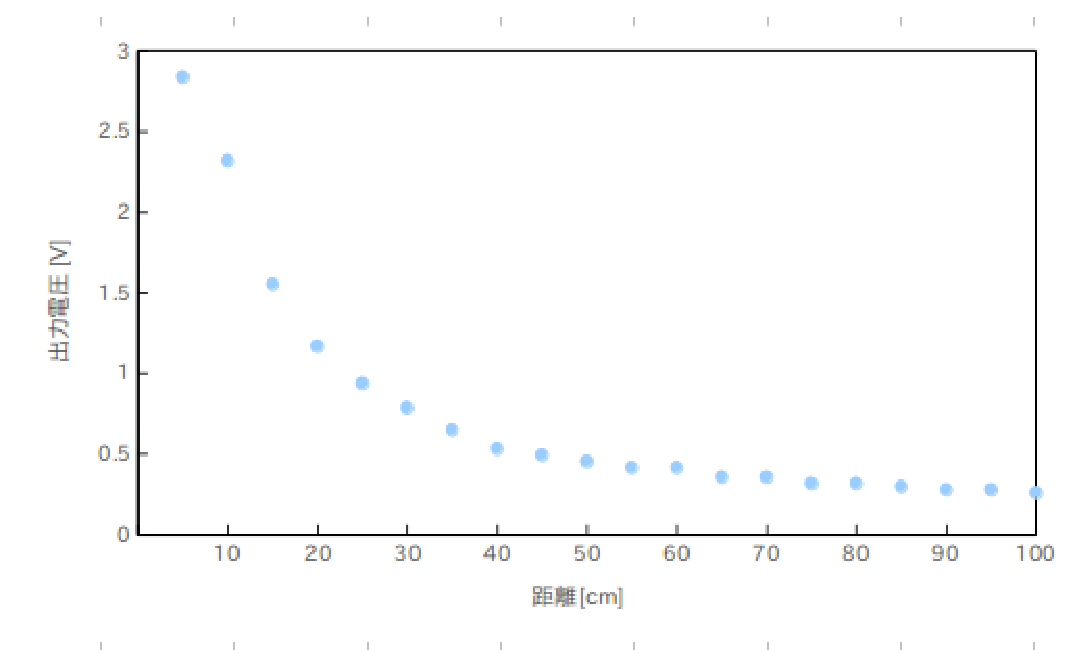
\includegraphics[width=1.0\hsize]{picture/psdn.eps}
    \caption{近距離センサ}
    \label{psdn}
  \end{center}
\end{figure}

\begin{figure}[H]
  \begin{center}
    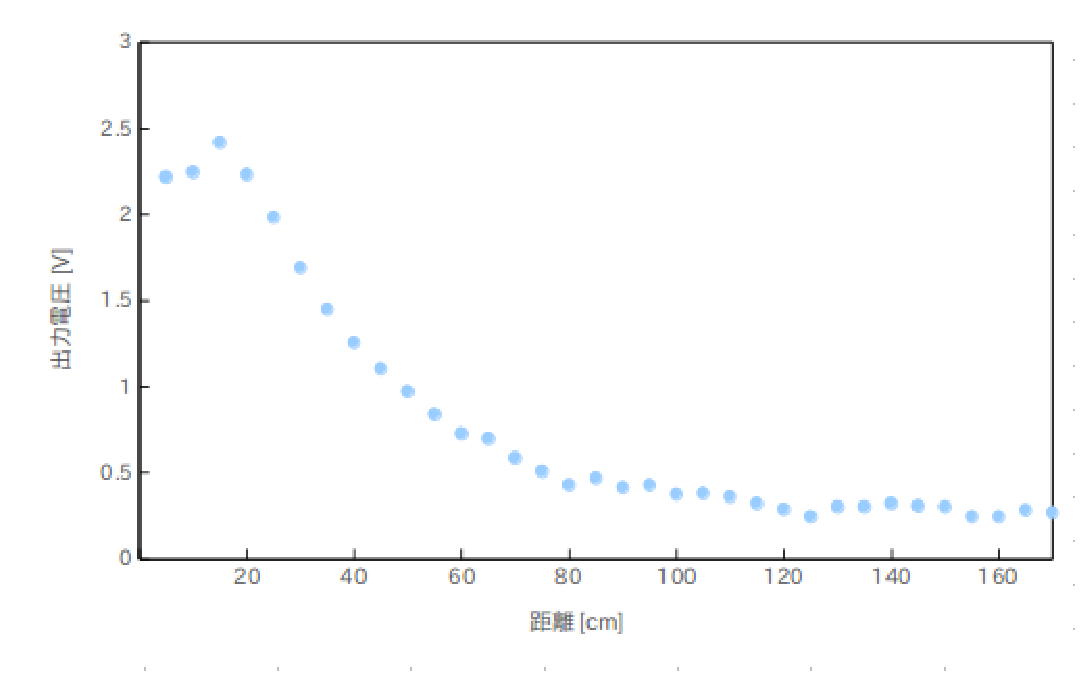
\includegraphics[width=1.0\hsize]{picture/psdf.eps}
    \caption{遠距離センサ}
    \label{psdf}
  \end{center}
\end{figure}


\newpage
\subsection{PSDセンサの課題}
今回のRCRにおいて用いるPSDセンサの課題として,
実験により得られた測定値のデータにノイズが入ることが挙げられる.
これを改善するためにフィルタをかけてノイズを除去することを考える.
ここでは以下の2種類のフィルタについてその実用性を考察する.
ただし,それらの検証実験は今後行うものとする.

\subsubsection{平均値フィルタ}
実測値の中で範囲を決めて,その平均値をとるフィルタのことである.
ノイズの影響を小さくすることができるが,フィルタが長くなると応答性能が悪化する.

\subsubsection{メディアンフィルタ(中間値フィルタ)}
奇数個のデータの中間に位置する値をその位置のデータとして
採用するフィルタのことである.スパイクノイズを取り除くのに適しているため,
今回使用するPSDセンサにはこちらのフィルタを用いることが適切であると考えられる.

\documentclass[11pt,a4j]{jarticle}

\input{include/macro.tex}
\input{include/preamble.tex}


\begin{document}
\section{機体の再設計}
\subsection{前回の反省}
前回のレポートで紹介した機体を図\ref{kuwano1}に示す.これを一号機とし,
一号機での反省点を元に再設計した機体を二号機とした.
二号機の概要を図\ref{kuwano2}に示す.一号機での反省点を以下に述べる.

\begin{itemize}
 \item 車体に無駄なスペースが多い.
 \item 車体の幅が大きい.
 \item 回路のガードがされていない.
\end{itemize}

西田研では,これらの反省点を改善するために,機体の大幅な見直しを行った.
改善した点について以下に述べていく.

\subsection{モータとエンコーダの配置}
一号機の駆動系を図\ref{kuwano3}に示す.一号機では,
モータとエンコーダの配置を線対称としていたため,
機体の幅が大きくしなければならなかった.そこで,
二号機ではこのモータとエンコーダの配置を点対象とすることにした.
これにより,タイヤのトレッド幅を限りなく小さくでき,
機体の幅を小さくすることができた.
また,一号機ではモータとエンコーダをアルミ板で下から支えるようになっていた.
そのため,モータとエンコーダを支える以外のスペースは無駄なスペースとなっていた.
二号機ではこの無駄なスペースを省くために,
モータとエンコーダを上から支えることにした.上から支えるにしたがって,
モータとエンコーダの重量と機体の荷重が図\ref{kuwano4}に示した部分に集中する恐れがあるため
,機体中心部分にモータおよびエンコーダを支えるパーツを3Dプリンタで作成し,
設置した.以上より,下から支えていたアルミ板を廃止することができ,
一号機での無駄なスペースを削減することができた.

\subsection{回路のガードについて}
機体の大部分はアルミでできているため,回路をそのままにしておくと,
ショートする可能性がある.したがって,回路をホットボンドで覆うことで
ショートすることを防ぐようにした.Arduinoに関しては専用のケースが存在しないため,
3Dプリンタでケースを作成した.

\subsection{タイヤについて}
一号機では図\ref{kuwano5}のようなタイヤを使用していたが,
このタイヤは中身がスポンジになっており,機体の重量でタイヤの接地面積が増えやすく,
また機体の荷重移動によって機体がロールする可能性があると考えた.
二号機ではそういった問題を解消するべく,ナロータイヤを使用することにした.
使用するナロータイヤを図\ref{kuwano6}に示す.使用するナロータイヤは非常に細いため,
地面との接地面積を少なくすることができる.また,ゴムのみでできているので,
一号機で使用する予定であったタイヤに比べて沈む量が少なく,
機体の荷重移動によるロールも低減できると考えられる.
しかし,接地面が小さくなったことでスリップする可能性があると考えられるので,
キャンバー角をつけるなどして対策を考えていく.

\begin{figure}[t]
  \begin{center}
    \includegraphics[width=1.0\hsize]{picture/kuwano1.eps}
    \caption{一号機}
    \label{kuwano1}
  \end{center}
\end{figure}

\begin{figure}[t]
  \begin{center}
    \includegraphics[width=1.0\hsize]{picture/kuwano2.eps}
    \caption{二号機}
    \label{kuwano2}
  \end{center}
\end{figure}

\begin{figure}[t]
  \begin{center}
    \includegraphics[width=1.0\hsize]{picture/kuwano3.eps}
    \caption{一号機の駆動系}
    \label{kuwano3}
  \end{center}
\end{figure}

\begin{figure}[t]
  \begin{center}
    \includegraphics[width=1.0\hsize]{picture/kuwano4.eps}
    \caption{最も荷重がかかる位置}
    \label{kuwano4}
  \end{center}
\end{figure}

\begin{figure}[t]
  \begin{center}
    \includegraphics[width=1.0\hsize]{picture/kuwano5.eps}
    \caption{一号機のタイヤ}
    \label{kuwano5}
  \end{center}
\end{figure}

\begin{figure}[t]
  \begin{center}
    \includegraphics[width=1.0\hsize]{picture/kuwano6.eps}
    \caption{二号機のナロータイヤ}
    \label{kuwano6}
  \end{center}
\end{figure}

\end{document}
\section{回路設計}
設計した回路について選定の理由や仕様について以下に示す.また使用する部品の一覧を\ref{tab:c_parts}に示す.
\subsection{マイコンの選定}
設計した回路を\ref{c_raspberry},\ref{c_arduino}に示す.
マイコンとして「Raspberry Pi3 Model B(以下 RPi)」と「Arduino uno R3(以下 Arduino)」を使用する.それぞれが,統合・画像処理・モータ制御,
センサ処理,を行う.RPiでは複雑な処理を行う上で,LinuxOSの支援を受けることができ有利である.さらに,処理速度がCPU 1.2[GHz],
メモリ1[GB]とArduinoの16[MHz]・32[KB]と比べても大きく優れている.これは,並列処理や高速な画像処理に適している.このような理由からRPi
を採用した.

また ,RPiはアナログI/Oポートを持っておらず,アナログ電圧出力を行うセンサ類の処理が困難である.そこで,アナログ・ディジタルI/Oポートを
持つArduinoにセンサ類の処理を担わせることとした.
\subsection{モータドライバ}
モータドライバは「MD10C R3」\ref{MD10C}を両輪駆動用として2つ使用し,「TA7291P」をアーム用として使用する.
各仕様を下に示す
.
[MD10C R3](駆動用)
\begin{itemize}
 \item モータ電源電圧 : DC 5[V]$〜$25[V]
 \item モータ最大電流 : 13[A]
 \item ロジック用電源 : モータ用より供給
 \item ロジック電圧   : DC 5[V] or 3.3[V]
\end{itemize}

[TA7291P](アーム用)
\begin{itemize}
 \item モータ電源電圧 : DC 0[V]$〜$20[V]
 \item モータ最大電流 : 1.0[A]
 \item ロジック電圧 : DC 4.5[V]$〜$20[V]
\end{itemize}
\begin{figure}[b]
 \centering
 \includegraphics[width=0.5\hsize]{../Circuit/picture/MD10C.eps}
    \caption{MD10C R3}
    \label{MD10C}
\end{figure}

\subsection{$I^2 C$通信}
今回,我々のロボットには測距センサを始めとする複数のセンサが搭載されている.これらの殆どがアナログ出力
であるが,ArduinoのアナログI/Oポートは6つしかなく,要求を満たしていない.

そこで,$I^2 C$通信を用いることとする.これは,$I^2 C$通信がパーティライン構成が可能となっており
,1つのマスタで複数のスレーブデバイスと通信することが可能であるからである.概要を以下に示す.
\begin{enumerate}
 \item マスタ側(Arduino)とスレーブ側(n個のセンサ等)を明確に分け,各スレーブに異なるアドレスを割り振る.
 \item マスタ側が、Start Conditionを出力し続いてアドレスとRead/Write要求を出力する.
 \item 全スレーブがこの時のSCLのクロックを元にSDAのデータを受信し、SSPADD
   レジスタにセットされたアドレスと一致したデバイスだけが、その後の送受信を
   継続する.
 \item 受信した側がデータを受信完了すると自動的にACKビットを返送し、同時にSSP割込みを発生する.
 \item これをマスタがStop Conditionを出力するまで続ける.
\end{enumerate}

\subsection{センサ仕様}
\subsubsection{赤外線測距センサ}  
測距センサは本体周囲に中距離用を7つ,前方に近距離用を3つ搭載する.これは自律行動の際に,
周辺環境,特に各種ポールを把握するために用いる. センサの仕様については実験を行ったので\ref{psdex}
 に示す.

また,各測距センサには信号のノイズを吸収し安定化させるために$0.1[\mu $F]のセラミックコンデンサを接続する.

\subsubsection{3軸加速度・ジャイロセンサモジュール}
加速度センサは[ x, y, z ]軸におけるロボットの加速度を測定するものである.

ジャイロセンサは[ x, y, z ]軸まわりの各加速度を測定するものである.

我々はこれらをロボットの自己位置推定に用いる.特にジャイロセンサについては,
ロボット本体の直進走行制御に使用する.詳細は\ref{algo}において説明する.
\begin{figure}[b]
 \centering
 \includegraphics[width=0.4\hsize]{../Circuit/picture/jairo.eps}
 \caption{3軸加速度・ジャイロセンサモジュール}
    \label{jairo}
\end{figure}
\subsection{電源回路}
電源回路は各回路図の左上に示している.\\
バッテリーはひとつしか搭載しないが,RPiとArduinoでは定格電流値が異なるために同一の電源は使用できない.
そこで,それぞれに降圧レギュレータとしてDCDCコンバータを用いてバッテリーからの供給電源を
分電することとした.各仕様を下に示す.


\begin{description}
 \item[【LR8697】(RPi・モータ用)] \mbox{} \\
	    電源電圧 : DC 6.0[V]$〜$42.0[V]] \\
	    出力電圧 : DC 5.0[V] \\
	    出力電流 : 2.5[A]
 \item[【BTD05-05S200D】(Arduino・センサ用)] \mbox{} \\
	    電源電圧 : 4.5$〜$9.0[V] \\
	    出力電圧 : 5.0[V] \\
	    出力電流 : 2000[mA]
\end{description}

\begin{table}[hb]
  \centering
  \caption{回路用部品表}
  \begin{tabular}{|c|c|r||c|} \hline
    タイプ & 部品名 & 数 & 用途 \\ \hline \hline
     マイコン & Raspberry Pi3 & 1& 統括・画像処理・モータ制御 \\ \cline{2-4}
     & Arduino uno R3& 1 & センサ類の処理 \\ \hline
     DCモータ & AO-8014 & 2 & 駆動用 \\ \cline{2-4}
      & TAMIYA ミニモータ & 1&アーム用  \\ \hline
    モータドライバ& MD10C-R3 & 2& タイヤ用 \\ \cline{2-4}
      &  TA7291P&1 &アーム用 \\ \hline
     赤外線測距センサ& GP2Y0A02YK &6&中距離センサ\\ \cline{2-4}
       &GP2Y0E03&3&近距離センサ \\ \hline
     カメラモジュール&P5V04A&1&画像処理\\ \hline
     3軸加速度センサ&KXR94-2050&1&自己位置推定\\ \hline
     3軸ジャイロセンサ&BGD20&1&自己位置推定\\ \hline
    DCDCコンバータ&LT8697&1& 7.2[V]→5.0[v]2500[mA]降圧レギュレータ\\ \cline{2-4}
       &BTD05-05S200D&1&7.2[V]→5.0[V]2000[mA]降圧レギュレータ\\ \hline
    コンデンサ&電解コンデンサ 47[$\mu$F]&2&電源安定化\\ \cline{2-4}
            &セラミックコンデンサ 0.1[$\mu$F]&9&センサ信号安定化\\ \hline
  バッテリー&POWER MAX 4000 Ni-MH&1&電源バッテリー 7.2[V]4200[mAh]\\ \hline
                 
  \end{tabular}
  \label{tab:c_parts}
\end{table}

\newpage
\begin{figure}[H]
 \centering
 \includegraphics[width=0.9\hsize]{../Circuit/picture/RCR_raspberryPi3.eps}
    \caption{Raspberry Pi3 接続回路図}
    \label{c_raspberry}
\end{figure}
\begin{figure}[H]
 \centering
 \includegraphics[width=0.9\hsize]{../Circuit/picture/RCR_arduino.eps}
    \caption{Arduino unoR3 接続回路図}
    \label{c_arduino}
\end{figure}

\documentclass[11pt,a4paper]{jsarticle}
\usepackage[dvips]{graphicx}
\usepackage{fancyhdr}
\usepackage{here}
\setcounter{page}{0}
%
\begin{document}

\section{自己位置推定}
ロボカーの中心が点$(x_k,y_k)$の位置にあるとし、時間$\Delta t$秒の間にロボカーが旋回中心の周りに$\Delta \theta$だけ回転したとする.このときロボカーの中心から車輪までの距離を$d$,左右の車輪とロボカーの中心が動いた距離をそれぞれ$\Delta L_R, \Delta L_L, \Delta L$とすると

\begin{eqnarray}
 \Delta L_R & = & (\rho + d)\Delta \theta \nonumber \\ 
 \Delta L_L & = & (\rho - d)\Delta \theta \nonumber \\
 \Delta L & = &\rho \Delta \theta
\end{eqnarray}

となる.これより

\end{document}

\newpage

\section{アルゴリズム}
3つのモードを切り替えながら完走する.
 \subsection{直線走行}
 まず最初の直線部分のアルゴリズムである.右斜め前についているPSDセンサが一定時間内にある閾値以上の反応を示す限り直進しする.そして車体右側についている2つのPSDセンサで同一のポールをとらえた時の測定距離の差を用いて車体のズレを検出し,車体角度を調節する.右斜め前についているPSDセンサが一定時間閾値以上の反応を見せなかった場合,右折し消火活動開始区間に入る.
 \subsection{消火エリア内}
火活動開始区間では一番近い入り口から順番にカメラで見ていく.ロボカーの侵入を妨げるポールがない入り口を見つけ次第すぐに消火エリアに入るように設定する.消火エリアに入ったのちすぐに左旋回しポール探索を行う.赤ポールを検出できたらそのポールまで行き消火活動を行う.消火したポールの先にまだ赤ポールがあるなら,そこまで行き消火する.その後Uターンし黄色ポールまでもどり,直線走行をする.一定距離,下に進んだのち左旋回し赤ポールを探索し消火する.これを繰り返し一番下まで探索を繰り返していく.
 \subsection{ゴールまで} 
色ポールに沿って下へ進んでいくが,その黄色ポールが検出できなくなると右旋回しゴールする.


\begin{figure}[hb]
\begin{center}
  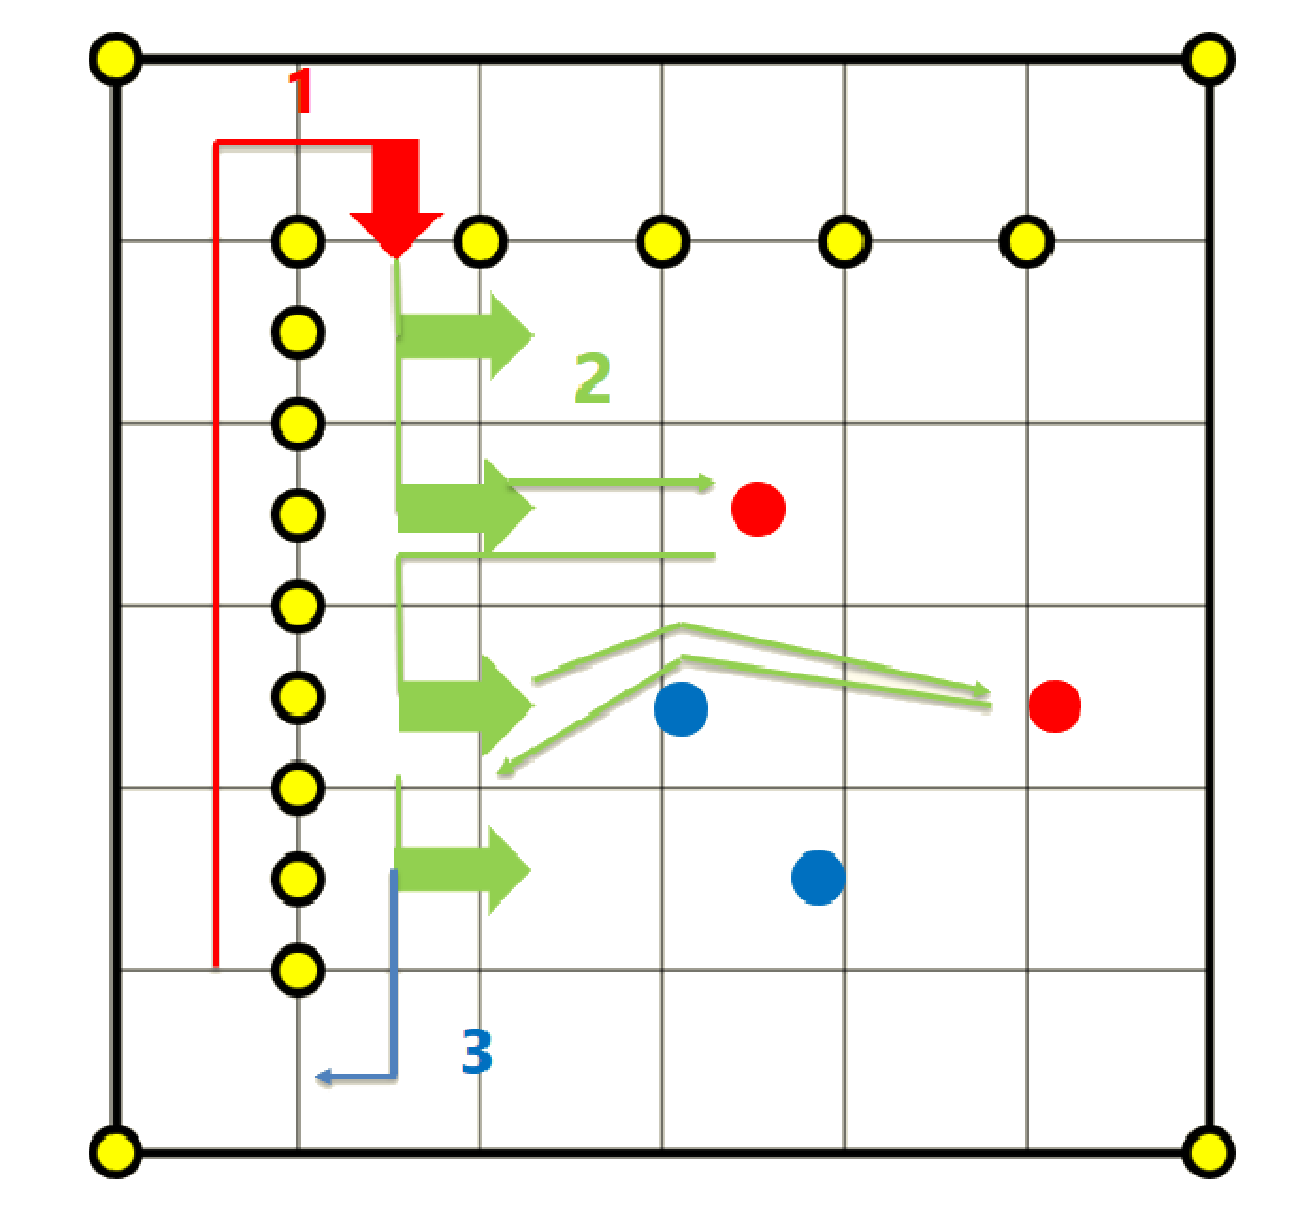
\includegraphics[scale = 0.4]{./picture/screen_shot.eps}
 \caption{アルゴリズム}
\end{center}
\end{figure}

\section{今後の予定}
図\ref{fig:schedule}に大まかな今後の予定を示す.
\begin{figure}[tH]
\begin{center}
  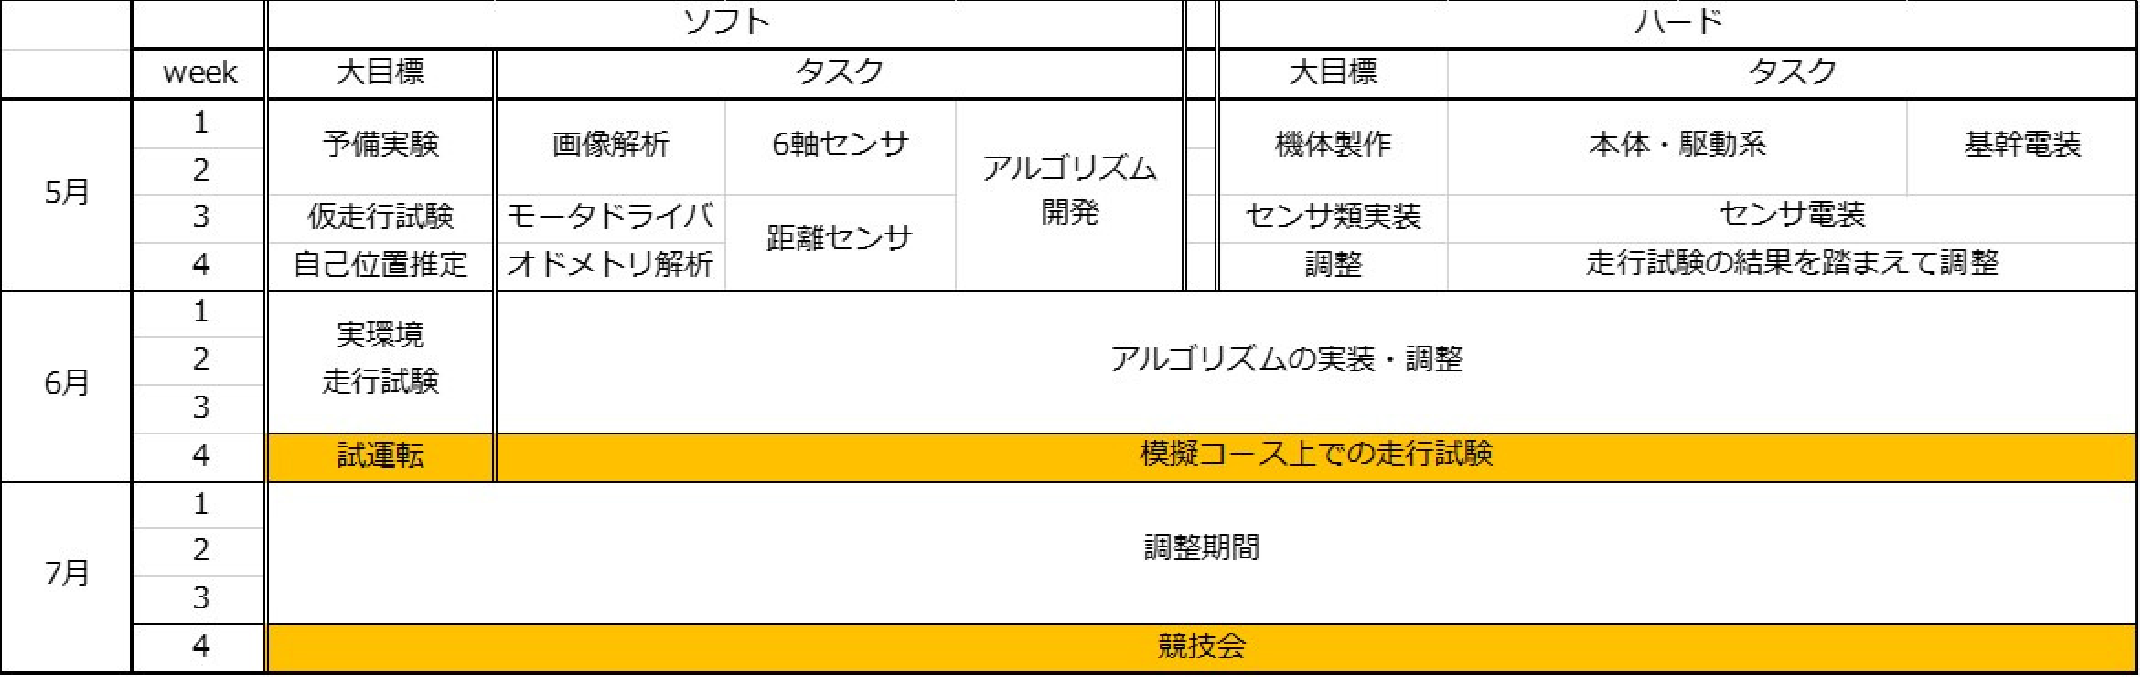
\includegraphics[width=1.0\hsize]{./picture/schedule.eps}
 \caption{今後の予定}
 \label{fig:schedule}
\end{center}
\end{figure}



\section{使用物品}
今回のRCRで使用する予定の物品を表\ref{tab:list1},\ref{tab:list2}に示す.4月26日時点での合計金額は78118円である.
\begin{table}[H]
 \begin{center}
  \caption{配布物品}
  \label{tab:list1}
  \begin{tabular}{|l|l|r|c|r|}  \hline
   メーカー & 商品名 & 単価 & 数量 & 価格 \\ \hline \hline 
   秋月電子通商 & ピンヘッダ(1X40) & 35円 & 1 & 35円  \\     \hline
   秋月電子通商 & ピンヘッダ(2X40) & 50円 & 1 & 50円  \\     \hline   
   秋月電子通商 & ソケット(2X40) & 95円 & 1 & 95円  \\     \hline
   秋月電子通商 & スミチューブ(黒) & 40円 & 1 & 40円 \\ \hline
   秋月電子通商 & スミチューブ(赤) & 40円 & 1 & 40円 \\ \hline
   秋月電子通商 & スミチューブ(クリア) & 40円 & 1 & 40円 \\ \hline
   秋月電子通商 & ハンダ & 280円 & 1 & 280円 \\ \hline
   秋月電子通商 & ハンダ吸い取り線 & 190円 & 1 & 190円 \\ \hline
   日本圧着端子 & XHベース 2極  & 10円 & 2 & 20円  \\     \hline
   日本圧着端子 & XHベース 3極  & 10円 & 7 & 70円  \\     \hline
   日本圧着端子 & XHベース 4極  & 10円 & 6 & 60円  \\     \hline
   日本圧着端子 & XHコネクタ 2極  & 10円 & 2 & 20円  \\     \hline
   日本圧着端子 & XHコネクタ 3極  & 10円 & 7 & 70円  \\     \hline
   日本圧着端子 & XHコネクタ 4極  & 10円 & 6 & 60円  \\     \hline
   日本圧着端子 & 圧着端子(XH)  & 4円 & 15 & 60円  \\     \hline
   光 & アルミ板 & 651円& 1& 651円\\ \hline
   &  & &合計 & 1130円  \\   \hline
  \end{tabular}
 \end{center}
\end{table}

\newpage

\begin{table}[H]
 \begin{center}
  \caption{引き継ぎ品}
  \label{tab:list1}
  \begin{tabular}{|l|l|r|c|r|}  \hline
   メーカー & 商品名 & 単価 & 数量 & 価格 \\ \hline \hline 
   TAMIYA & タミヤギヤードモータ & 4860円 & 2 & 9720円  \\     \hline
   TAMIYA & ギヤードモータハブシャフトセット & 540円 & 1 & 9720円   \\  \hline
   TAMIYA & ミディアムナローレーシンググラジアルタイヤ & 540円 & 1 & 540円  \\  \hline
   TAMIYA & ミディアムナロー5本スパークホイール & 540円 & 1 & 540円   \\     \hline
   TAMIYA & SP.106 7.2Vコネクタ & 270円 & 2 & 540円  \\      \hline
   RSコンポーネンツ株式会社 & カメラモジュール &  2740円 & 1 & 2740円  \\ \hline
   RSコンポーネンツ株式会社 & Rasberry Pi 3 ケース & 1080円 & 1 & 1080円  \\    \hline
   RSコンポーネンツ株式会社 & Raspberry Pi 3 Model B & 6200円 & 1 & 6200円  \\     \hline
   MISUMI & トグルスイッチ & 80円 & 2 & 160円 \\       \hline
   MISUMI & キャスターホイール & 990円 & 1 & 990円 \\     \hline
   KHK & 歯車(モジュール 0.5 歯数60) &1360円 & 4 & 5440円 \\      \hline
   KHK & プラスチックナット+連結スペーサーセット & 100円 & 1 & 100円  \\      \hline
   秋月電子通商 & 3軸加速度センサモジュール & 850円 & 1 & 850円  \\     \hline
   秋月電子通商 & 3軸ジャイロセンサモジュール & 750円  & 1 & 750円 \\     \hline
   Cytron &DCブラシモータドライバ & 2160円 & 2 & 4320円 \\       \hline
   Powers & POWER MAX 4000 Ni-MH& 4000円 & 2 & 8000円  \\     \hline
   シャープ株式会社 & シャープ測距モジュール & 400円 & 6 & 2400円  \\    \hline
   株式会社矢島製作所 & ユニバーサル基盤 & 100円 & 2 & 200円 \\    \hline
   日本電産コパル電子 & ロータリエンコーダ & 7500円 & 2 & 15000円  \\   \hline
   Arduino Srl & Arduino UNO & 3240円 & 1 & 3240円  \\     \hline
   TOSHIBA & microSDHC メモリーカード 8GB & 1058円 & 1 & 1058円  \\    \hline
   OptoSupply & スペーサー & 45円 & 4 & 180円  \\     \hline
   GWS &サーボモータ & 1000円 & 1 & 1000円  \\    \hline
   ルビコン株式会社 & 電解コンデンサ(47μF) & 10円 & 2 &20円 \\     \hline
   &  & &合計 & 65608円  \\   \hline
  \end{tabular}
 \end{center}
\end{table}

\newpage
\begin{table}[H]
 \begin{center}
  \caption{新規購入品}
  \label{tab:list2}
  \begin{tabular}{|l|l|l|r|c|r|}  \hline
   取引先 & 商品名 & 型番または商品コード & 単価 & 数量 & 価格 \\   \hline \hline
   Strawberry Linux & 近距離センサモジュール & VL6180X & 1296円 & 3 & 3888円 \\    \hline
   Strawberry Linux & 降圧型DC-DCコンバータ & LT8697 & 1404円 & 1 & 1404円  \\      \hline
   スイッチサイエンス & アナログマルチプレクサ & 767円 & 1 &767円 & \\ \hline
   秋月電子通商 & シャープ測距モジュール & GP2Y0E03 & 760円 & 1 & 760円  \\      \hline
   秋月電子通商 & I2Cバス用双方向レベル変換モジュール & PCA9306 & 150円 & 1 & 150円  \\      \hline
   misumi & 小径玉軸受 & FL686ZZ & 440円 & 4 & 1760円  \\      \hline
   misumi & イグリデュールG フランジ型軸受 & GFM-0608-25 & 75円 & 5 & 375円 \\     \hline
   misumi & アルミ 角パイプ & HFHQ1515-1.5-500 & 200円 & 1 & 200円  \\       \hline
   秋月電子通商 & モータドライバ & TA7291P & 300円 & 1 & 300円  \\    \hline
   横山テクノ & アルミ 丸パイプ 6×1.0×400 & & 310円 & 1 & 310円 \\    \hline
   ヨドバシカメラ & ミニモータ低速ギアボックス & 70189 & 716円 & 1 & 716円  \\   \hline
   & & & & 合計 & 11610円  \\      \hline
  \end{tabular}
 \end{center}
\end{table}


\newpage
\setcounter{page}{1}
\pagestyle{fancy}
\renewcommand{\headrulewidth}{0.0pt}
\rhead{付録\thepage}
\lhead{}
\cfoot{}
\input{./appendix.tex}


\end{document}
